\documentclass[12pt]{article}
\usepackage{setspace, indentfirst, graphicx, enumerate, authblk}
\usepackage[vmargin=3.18cm,hmargin=2.54cm]{geometry}
\sloppy	% better line breaks
\title{Social Network Search Engine}
\author{Yow-Bang Wang\\
\texttt{ybdarrenwang@gmail.com}}

\begin{document}
\maketitle

{\footnotesize
\noindent
Copyright (c) 2012, Yow-Bang Wang and Yung-Hsiang Yang\\
All rights reserved.\\
\\
Redistribution and use in source and binary forms, with or without modification, are permitted provided that the following conditions are met:\\
1. Redistributions of source code must retain the above copyright notice, this list of conditions and the following disclaimer.\\
2. Redistributions in binary form must reproduce the above copyright notice, this list of conditions and the following disclaimer in the documentation and/or other materials provided with the distribution.\\
3. Neither the name of the copyright holders nor the names of its contributors may be used to endorse or promote products derived from this software without specific prior written permission.\\
\\
THIS SOFTWARE IS PROVIDED BY THE COPYRIGHT HOLDERS AND CONTRIBUTORS "AS IS" AND ANY EXPRESS OR IMPLIED WARRANTIES, INCLUDING, BUT NOT LIMITED TO, THE IMPLIED WARRANTIES OF MERCHANTABILITY AND FITNESS FOR A PARTICULAR PURPOSE ARE DISCLAIMED. IN NO EVENT SHALL THE COPYRIGHT HOLDER OR CONTRIBUTORS BE LIABLE FOR ANY DIRECT, INDIRECT, INCIDENTAL, SPECIAL, EXEMPLARY, OR CONSEQUENTIAL DAMAGES (INCLUDING, BUT NOT LIMITED TO, PROCUREMENT OF SUBSTITUTE GOODS OR SERVICES; LOSS OF USE, DATA, OR PROFITS; OR BUSINESS INTERRUPTION) HOWEVER CAUSED AND ON ANY THEORY OF LIABILITY, WHETHER IN CONTRACT, STRICT LIABILITY, OR TORT (INCLUDING NEGLIGENCE OR OTHERWISE) ARISING IN ANY WAY OUT OF THE USE OF THIS SOFTWARE, EVEN IF ADVISED OF THE POSSIBILITY OF SUCH DAMAGE.\\
}

\section*{Developed by:}
\noindent
(Darren) Yow-Bang Wang, Graduate Institute of Electrical Engineering, NTU.\\
(Larry) Yung-Hsiang Yang, Graduate Institute of Computer Science and Information Engineering, NTU.\\

\section{Introduction}

This is my final project of grad-school class "Design Pattern and Software Development" of National Taiwan University (NTU) in Spring 2012. This project is done in pair-programming. My partner (Yung-Hsiang Yang, Git ID: larry61410) was mainly in charge of the implementation of API calls to social networks. And I (Yow-Bang Wang, Git ID: piscesfantasy) was in charge of framework design the remaining implementations. In this project we implemented a social network search engine with C++ and Python. The first version support search on Plurk and Twitter. Main functions include keyword/friend search, browsing search results, recommendation and reply.

\section{Compilation}

The makefile in the main file directory have been tested for g++ complier under Linux and MacOS.
\begin{enumerate}
\item {\it make} or {\it make all}: constructs the binary executable "SocialNetworkSearchEngine.exe".
\item {\it make clean}: remove the "build" folder and all the .o files inside.
\item {\it make doc}: if you have installed Doxygen and GraphViz, this command will generate HTML document inside "doc" folder. 
\end{enumerate}

\section{Execution}

In this section we will demonstrate how to run this program {\it SocialNetworkSearchEngine.exe} if you already have a Plurk account. For Twitter the same procedure should apply too.

\subsection{Preparation}

The folders "Plurk" and "Twitter" contains python scripts that will be called. Therefore to run this program, the folders "Plurk" and "Twitter" must be in the same directory.

We use the following Python libraries for Social Network API:
\begin{enumerate}
\item Plurk: plurk-oauth by clsung, available at http://www.plurk.com/API
\item Twitter: tweepy by joshthecoder, available at https://dev.twitter.com/docs/api
\end{enumerate}

\subsection{Login}

This program adopts interactive command line interface. For the first execution of {\it SocialNetworkSearchEngine.exe} you will see the messages below:

\begin{table}[!h]
\centering
\vspace{2mm}
\centerline{
\begin{tabular}{|l|}
\hline
Initializing Twitter\\
Initializing Plurk\\
Warning: can't load query history log\\
Choose Social Network (type "exit" to quit): \\
$>$ \\
\hline
\end{tabular}}
\end{table}

Just type "Plurk" If you want to login Plurk (the initial must be upper case!) and press enter. Then you can input your id and password. If this is your first login with this program, after entering ID and password you will see something like this:

\begin{table}[!h]
\centering
\vspace{2mm}
\centerline{
\begin{tabular}{|l|}
\hline
Open the following URL and authorize it\\
http://www.plurk.com/OAuth/authorize?oauth\_token=......\\
Input the verification number: \\
\hline
\end{tabular}}
\end{table}

Browse the authentication webpage to get the verification number. This procedure will run twice to get required access token, and the program would store the access token in the file "API\_plurk\_all.keys" and "API\_twitter.keys" in current directory.

\subsubsection{Password Masking}
Note we have also implemented Password Masking. However, this function was done by POSIX, which means this function is valid only under Linux environment.

\subsection{Search}

After logging in you will see this:
\begin{table}[!h]
\centering
\vspace{2mm}
\centerline{
\begin{tabular}{|l|}
\hline
Start the next query? [y/n]: \\
$>$ \\
\hline
\end{tabular}}
\end{table}

You can choose "n" to logout, or choose "y" to begin a search. The program will ask if you need "Basic Search" or "Advanced Search":
\begin{table}[!h]
\centering
\vspace{2mm}
\centerline{
\begin{tabular}{|l|}
\hline
Choose query mode (1.Basic, 2.Advanced): \\
$> $\\
\hline
\end{tabular}}
\end{table}

\begin{enumerate}
\item Basic Search: Search over all the public messages with a keyword.
\item Advanced Search: Search over all the messages of your friends with a keyword and a friend's ID.
\end{enumerate}

\subsubsection{Auto-complete}

While entering either keyword or a friend's ID, this program also support auto-complete. For keyword the program will search and iterate through your most recent 100 queries stored in the file "queryHistory.log" in current folder; and for friend's ID the program will search and iterate through your friend lis stored in the file "FriendsList" in current folder. 

Yet for now this function is normal only for English words. There may be some unexpected error if you try to auto-complete non-English words.

\subsection{Browse, Recommend and Reply}

After entering your query, the program will retrieve relevant posts and store them in the file "POST.json" in current folder. The first post will be shown on the screen followed by some options:
\begin{table}[!h]
\centering
\vspace{2mm}
\centerline{
\begin{tabular}{|l|}
\hline
Whats next?\\
- Pu this post [l]\\
- Reply this post [r]\\
- Go to next post [n]\\
- Quit browsing [q]\\
\hline
\end{tabular}}
\end{table}

If you are browsing posts except the first one, the option will also includes:
\begin{table}[!h]
\centering
\vspace{2mm}
\centerline{
\begin{tabular}{|l|}
\hline
- Go to previous post [p]\\
\hline
\end{tabular}}
\end{table}

Just enter the option in the bracket to execute.

\subsection{Terminate}

To terminate the program, just type "exit" when you are not logged in any social network.

\section{System Framework and Design Patterns}

\begin{figure}[t]
\centering
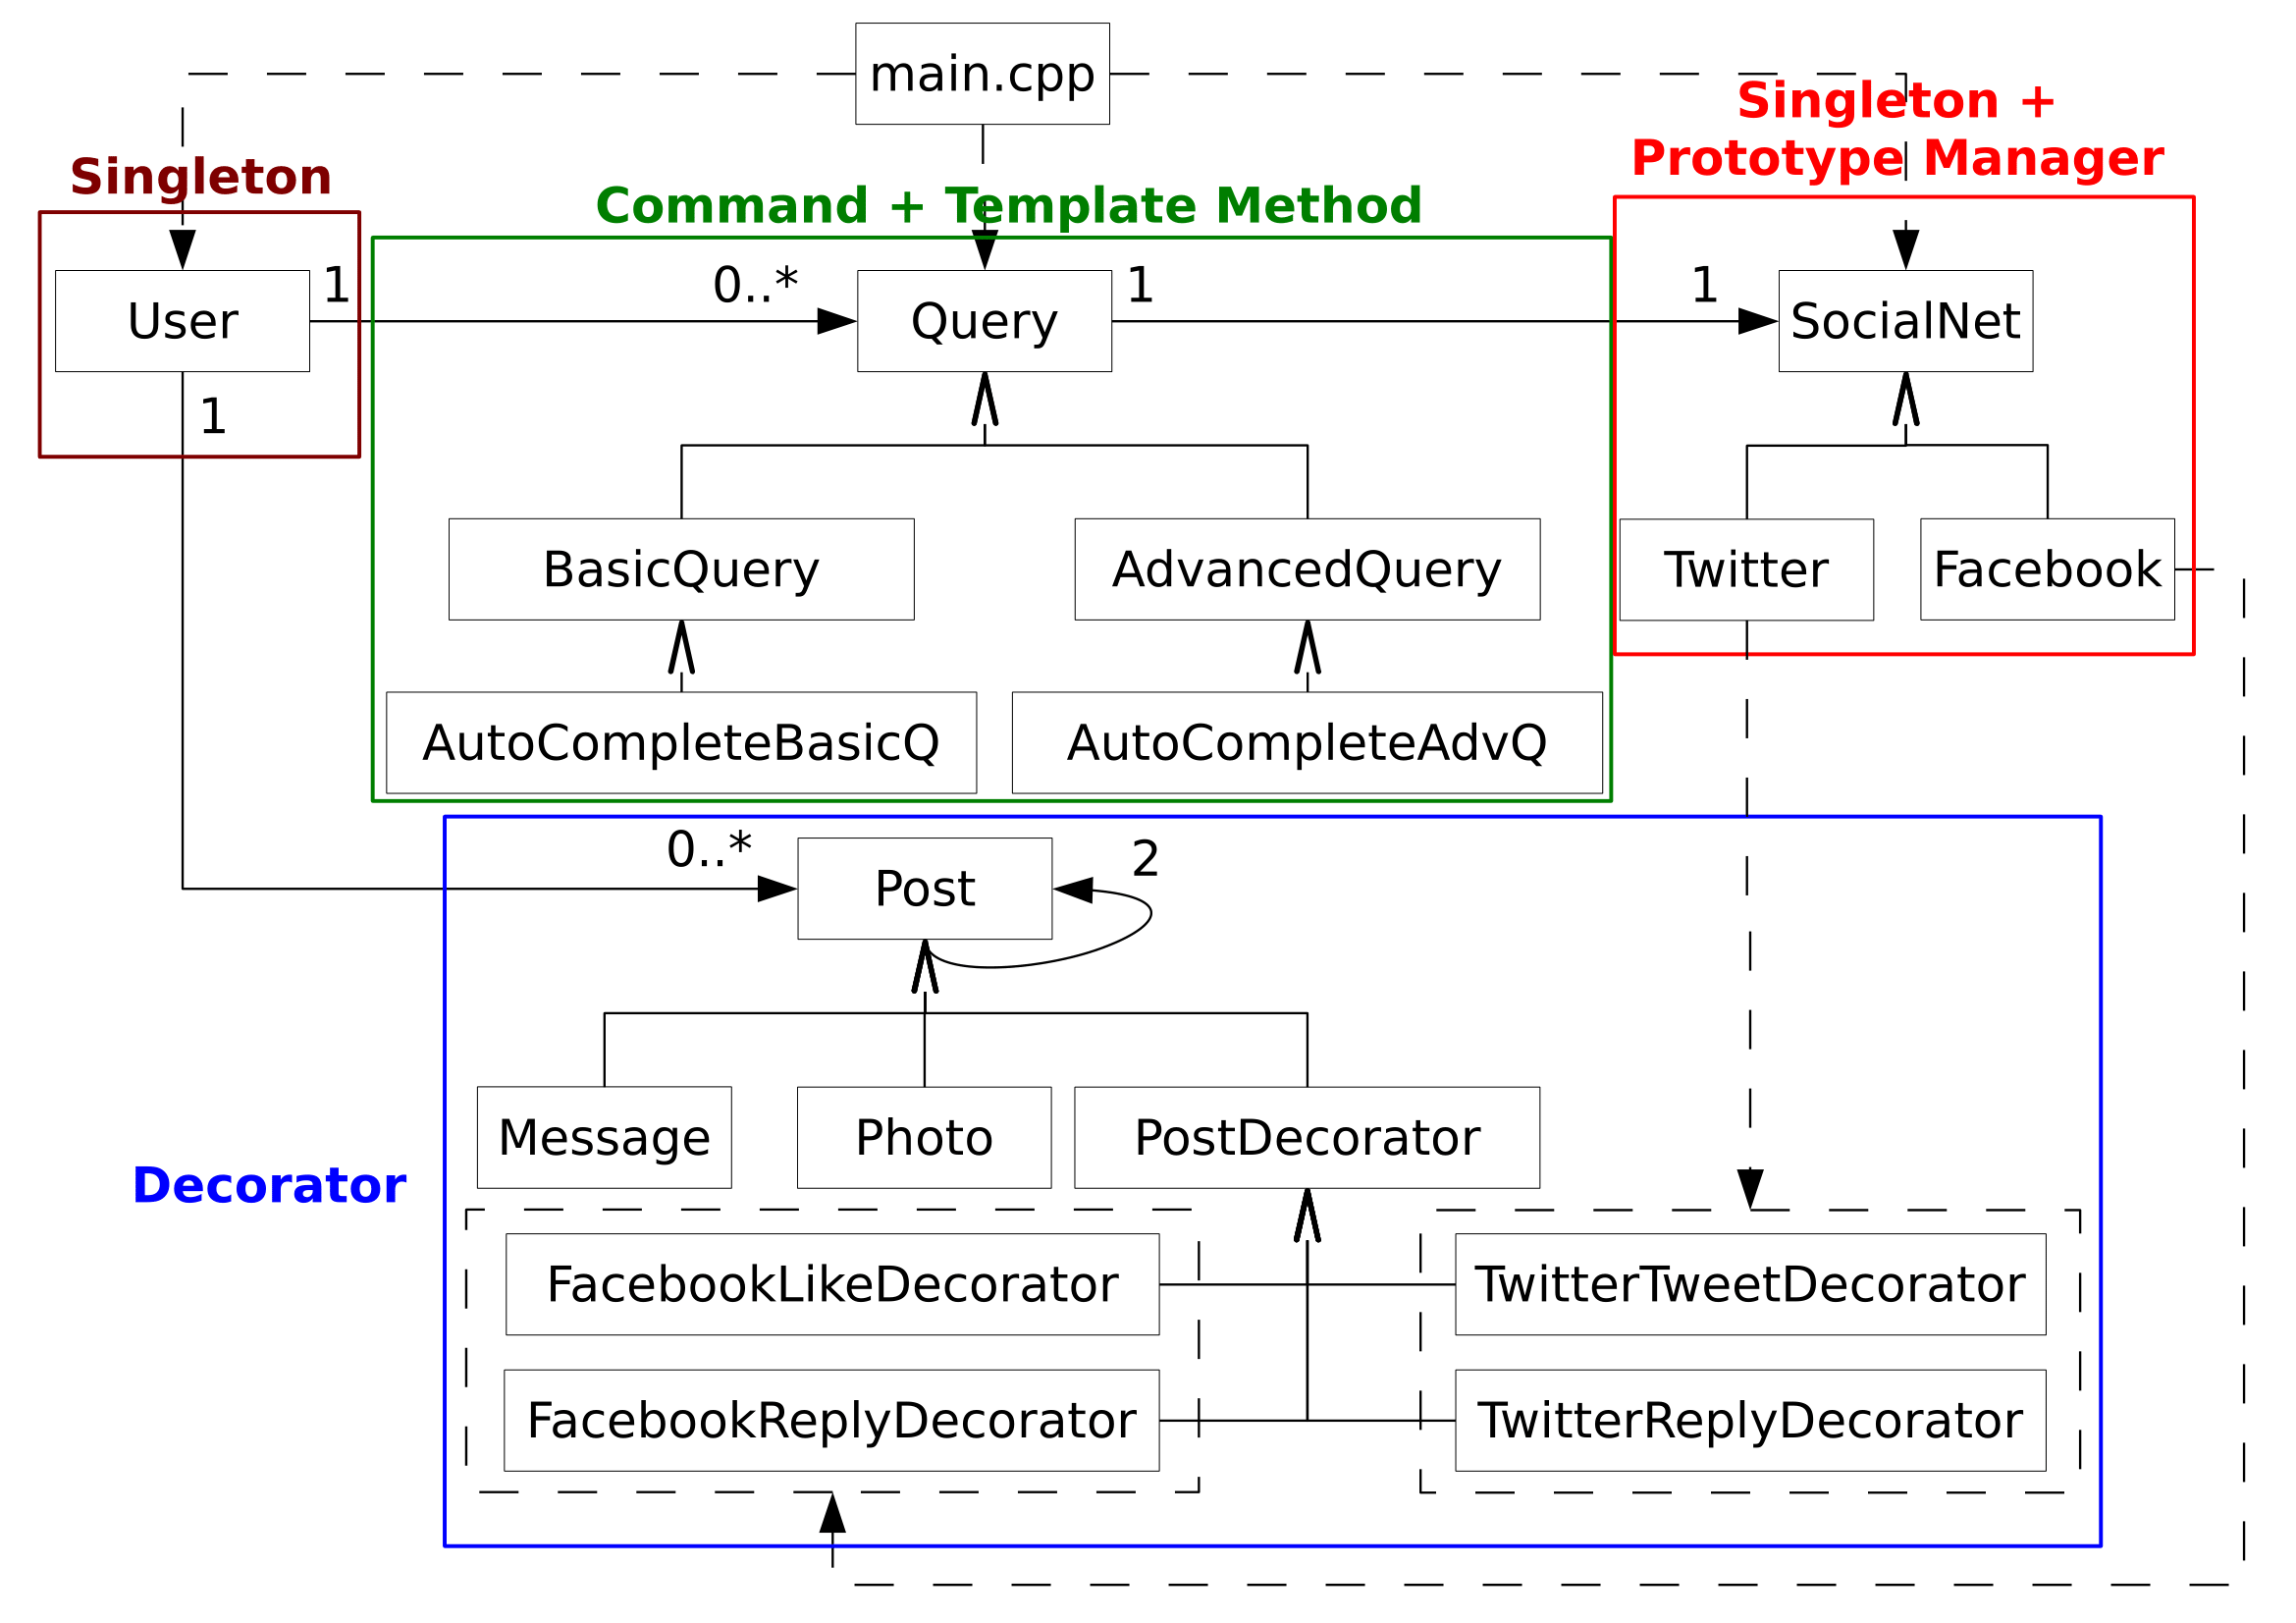
\includegraphics[width=15cm]{doc/classDiagram}
\caption{{\it The framework of our program}}
\label{fig:classDiagram}
\end{figure}

Fig. \ref{fig:classDiagram} shows the overall framework of this program. There are several design patterns involved:
\begin{enumerate}
\item class User: Singleton
\item class SocialNet: Singleton + Prototype Manager + Abstract Factory
\item class Query: Command + Template Method
\item class Post: Decorator 
\end{enumerate}
For more details please refer to "doc/designPattern.pdf".

\end{document}
